\documentclass{article}
\usepackage[a4paper, margin=1in]{geometry}
\usepackage[T1]{fontenc}
\usepackage[utf8x]{inputenc}
\usepackage{ucs}
\usepackage{xhfill}
\usepackage[spanish]{babel}
\usepackage{url}
\usepackage{tikz}  
\usepackage{fancyhdr}
%\usepackage[landscape]{geometry}
\usepackage{amsmath,amsthm,amssymb} 
\usepackage{mathrsfs}
\usepackage{dsfont}
\usepackage{upgreek}
\usepackage{graphicx}
\usepackage{svg}
\usepackage{listings}
\usepackage{rotating}
\usepackage{color} 
\usepackage{wasysym}
\usepackage{hyperref}
\usepackage{multicol}

\definecolor{codegreen}{rgb}{0.08, 0.65, 0.24} 
\definecolor{codewine}{rgb}{0.5, 0.0, 0.5}
\definecolor{codegray}{rgb}{0.63, 0.63, 0.63}
\definecolor{codeblue}{rgb}{0.15, 0.31, 0.78}
\definecolor{backcolour}{rgb}{0.97, 0.97, 0.97}

\lstdefinestyle{villalpando}{
  backgroundcolor=\color{backcolour},   
  commentstyle=\color{codewine},
  keywordstyle=\color{codegreen},
  numberstyle=\tiny\color{codegray},
  stringstyle=\color{codeblue},
  basicstyle=\footnotesize,
  breakatwhitespace=false,         
  breaklines=true,                 
  keepspaces=true,                 
  numbers=left,                    
  numbersep=5pt,                  
  showspaces=false,                
  showstringspaces=false,
  showtabs=false,                  
  tabsize=2
} 
\lstset{style=villalpando}

\pagestyle{fancy}
\fancyhf{}
\renewcommand{\headrulewidth}{0pt}
\lhead{}
\chead{}
\rhead{}
\lfoot{}
\cfoot{\itshape diego.a.villalpando@ciencias.unam.mx}
\rfoot{\thepage}

\begin{document}

%===========Título===========%

{\centering 
\noindent\hrulefill \par \vspace{0.5cm}
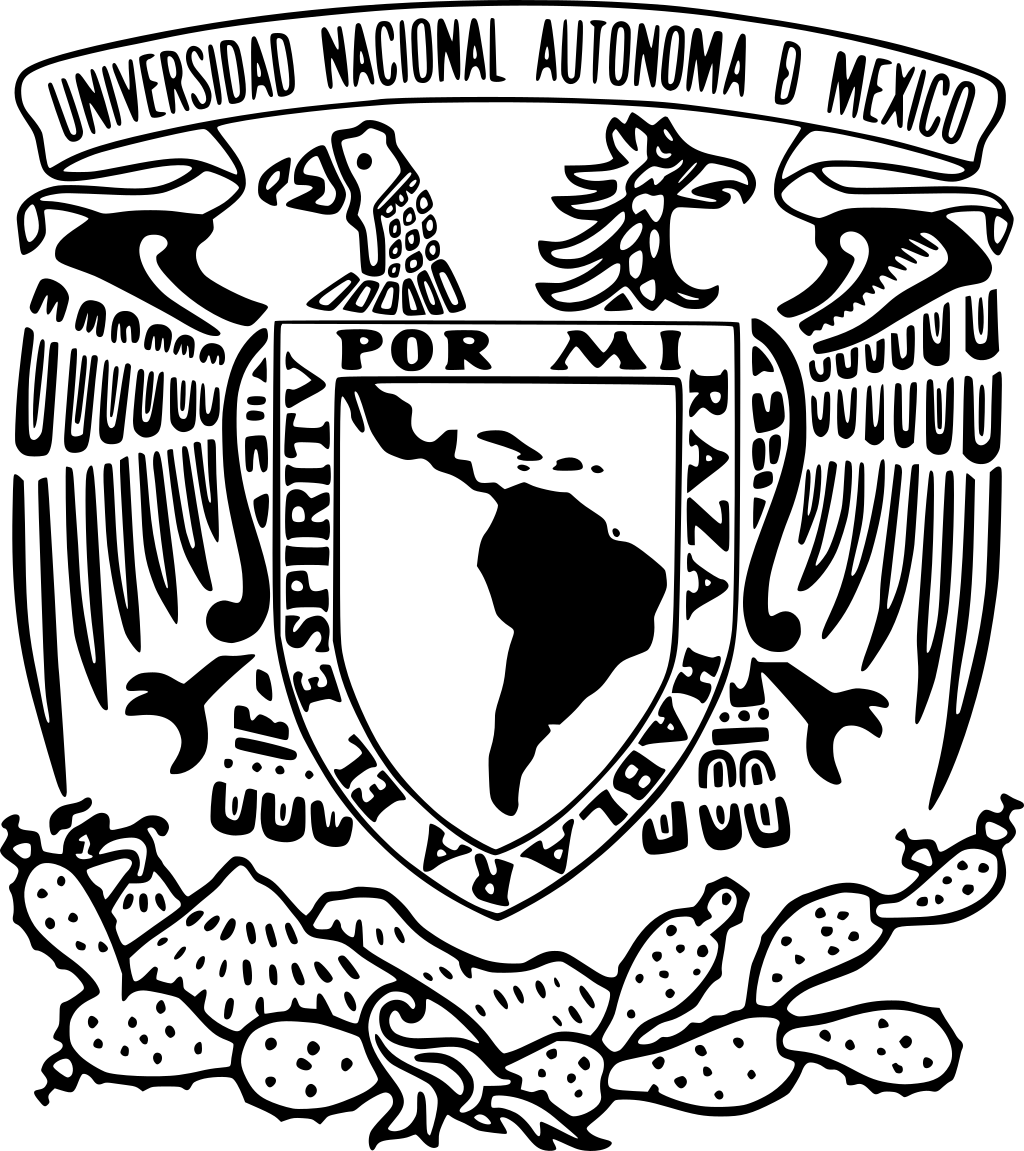
\includegraphics[width=2cm]{unam.png} \hspace{11.5cm}
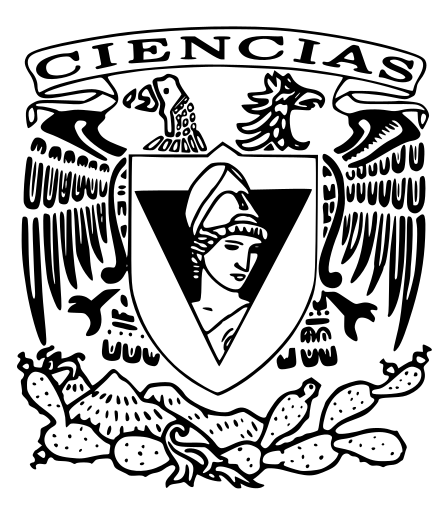
\includegraphics[width=2cm]{ciencias.png}\vspace{-2.2cm}
     {\scshape\Large Universidad Nacional Autónoma de México \par}
     {\scshape\Large Facultad de Ciencias, Ciudad Universitaria \par}
     {\Large Fundamentos de Bases de Datos 7063\par}
     \vspace{0.2cm}
     {\Large\bfseries Diseño de Base de Datos Caso de Uso \par}
     \vspace{0.2cm}
     {\large\itshape Diego Alfredo Villalpando Velázquez \par \vspace{0.2cm}}
     {\large\itshape 13 de diciembre de 2019\par} \vspace{0.35cm}
     \noindent\hrulefill
}

%===========Objetivo===========%
\vspace{0.5cm}
       { \bfseries
         Objetivo:
         Se describe a continuación el esquema de la base de datos basada en Postgresql 10
         sobre el caso de uso: la empresa Transpórtate. Con el uso de diagramas
         entidad/relación, diagramas relacionales, esquema de las tablas de dicha base de
         datos, y sus respectivas justificaciones.
       }
       
       % Índice de contenido
       \noindent \tableofcontents
       
       %===========Introducción===========%
       \newpage
       \section{Introducción}
               {
                 La empresa Transportate es una empresa de transporte particular con 150 automóviles
                 propios para transporte de usuarios ajenos a la empresa y de forma individual. La
                 empresa desea crear una base de datos que permita realizar estadísticas
                 de los viajes e implementar un nuevo sistema de recompensas para sus clientes
                 frecuentes. Se enumeran las reglas de negocio a continuación:
               }
               
               {\begin{itemize}
                 \item Se deberán almacenar los datos básicos de los clientes: nombre completo, di-
                   rección, correo(s) electrónico(s), teléfono(s), fecha de nacimiento y todos los
                   otros datos que se considere relevante para la correcta funcionalidad del sistema.
                   
                 \item A cada cliente se le debe otorgar una tarjeta de cliente digital frecuente para
                   acumular sus puntos.
                   
                 \item Cada punto acumulado en la tarjeta digital tendrá un valor de 10 centavos, de
                   manera que 10 puntos se podrán utilizar como 1 peso, mismos que podrás usar
                   para pagar viajes posteriores.
                   
                 \item Se desea implementar un programa para realizar distintos tipos de viajes, viajes
                   compartidos los cuales tendrían una tarifa mas económica o viajes privados
                   con una tarifa mas elevada.
                   
                 \item Adicional a esto los automóviles los quieres clasificar por categorías:
                   \begin{enumerate}
                   \item Luxury: Son viajes en autos lujosos, que tienen un costos de mas de 450,000.00
                     MXM. Estos autos solo pueden ser rentados para los viajes de tipo privado.
                   \item Lite: Son viajes en autos normales, que tienen un costos de a lo mas de
                     449,000.00 MXM. Estos autos pueden ser rentados para los viajes de tipo
                     privado o compartido.
                   \item Luxury SUV: Son viajes en autos para mas de 5 pasajeros y tienen es-
                     tos automóviles un costos de mas de 500,000.00 MXM. Estos autos solo
                     pueden ser rentados para los viajes de tipo privado.
                   \end{enumerate}

                 \item En el caso de los automóviles, las características que se desean almacenar en
                   cada uno son: precio de factura, placas, marca, submarca, año, color.
                   
                 \item Para los viajes que se realizan, se requiere un informe detallado de cada uno
                   en donde se solicito (origen), destino final , nombre del chofer, las placas del
                   automóvil, tiempo del viaje, costo del viaje, forma de pago.
                   
                 \item Se debe de registrar la forma en la que se realizo el pago del viaje, el pago pue-
                   de ser cualquiera de las siguientes combinaciones: efectivo, tarjeta de crédito,
                   débito o tarjeta digital de puntos.
                   
                 \item La compra podrá ser cubierta parcial o totalmente con el saldo del monedero, sin
                   embargo, tras la compra se deberán abonar los puntos generados por ésta.
                   
                 \item Para los choferes se requiere almacenar su información básica así como su in-
                   formación personal. Interesa además saber el automóvil que le toca al chofer ya
                   que le puede ir tocando diferentes automóviles por semana.
                   
                 \item De acuerdo a la ubicación de las personas que solicitan un viaje es importante
                   saber a que automóvil se debiera enviar, ya que se tendría que buscar el que se
                   encuentre mas cercano.
               \end{itemize}}
       
       %===========Diseño E/R===========%
       \section{Modelo Entidad/Relación del Caso}

       \subsection{Diagrama}

       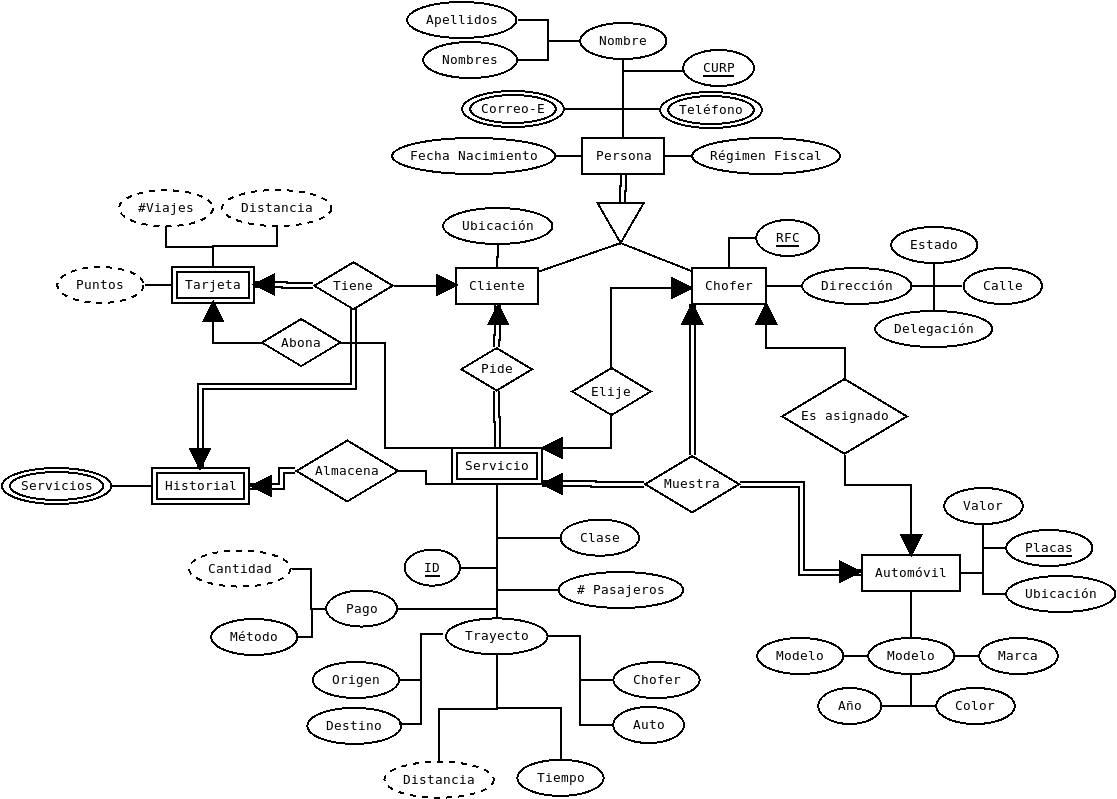
\includegraphics[width=14.7cm]{ER.png}\\
       \centerline{Diagrama 1: Modelo Entidad-Relación del caso.}

       \subsection{Justificación}

       { 
       Se consideró: que Clientes y Choferes deben ser herederos de Persona, ya que tienen muchos
       atributos en común, y es el mismo tipo de objeto pero con la diferencia de uno ser parte de
       la empresa. Además, que debe existir un objeto Servicio el cual relacione el pedido de los
       Clientes con las acciones de la empresa para solucionar su pedido. También, que los atributos
       de Tarjeta: Puntos, $\#$Viajes, Distancia; así como los de Servicio:
       Cantidad, y Distancia; son atributos calculados automáticamente en función de los datos
       ingresados en Servicio.
       }\\

       { \noindent
         \subsubsection*{Relaciones}
         \begin{multicols}{2}
           \begin{itemize}
           \item Un Cliente tiene una Tarjeta.
           \item Un Cliente tiene un Historial.
           \item Un Cliente pide un Servicio.
             
           \item Un Chofer es asignado a un Automóvil.
             
           \item Un Automóvil es asignado a un Chofer.
             
           \item Un Servicio elije un Chofer.
           \item Un Servicio muestra un Chofer.
           \item Un Servicio muestra un Automóvil.
           \item Un Servicio es almacenado en un Historial. 
           \item Un Servicio abona una Tarjeta.        
           \end{itemize}
         \end{multicols}
       }
       
       { \noindent
         \subsubsection*{Llaves}
         \begin{multicols}{2}
           \begin{itemize}
           \item Cliente: CURP.
           \item Chofer: RFC, CURP.
           \item Automóvil: Placas.
           \item Servicio: ID.
           \end{itemize}
         \end{multicols}
       }
       
       { \noindent
         \subsubsection*{Discriminantes}
         \begin{multicols}{2}
           \begin{itemize}
           \item Tarjeta: Distancia, Puntos, $\#$Viajes.
           \item Historial: Servicios.
           \end{itemize}
         \end{multicols}
       }
       
       
       
       %===========Diseño Relacional===========%
       \section{Modelo Relacional del Caso}
       
       \subsection{Diagrama}
       
       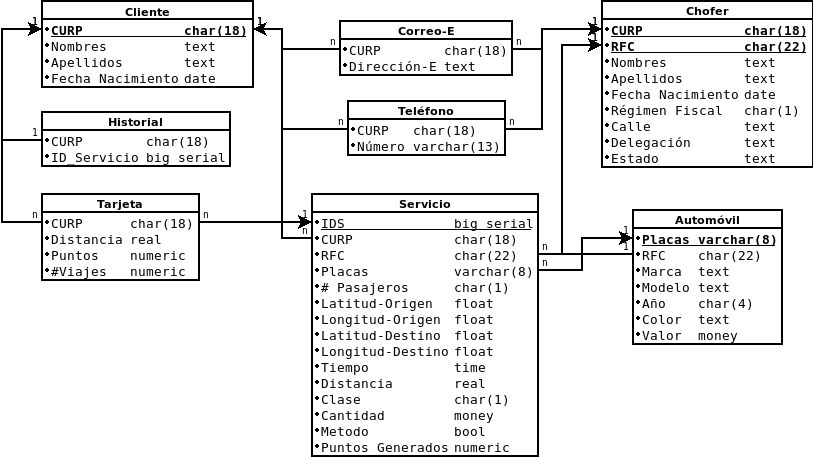
\includegraphics[width=15cm]{R.png}\\
       \centerline{Diagrama 2: Modelo Relacional del caso.}
       
       \subsection{Justificación}
       
       { \noindent
         \subsubsection*{Dependencias Funcionales}
           \begin{itemize}
           \item Cliente ( CURP $\rightarrow$ Nombres, Apellidos, Fecha Nacimiento )
             
           \item Historial ( CURP $\rightarrow$ IDS )
             
           \item Tarjeta ( CURP $\rightarrow$ Distancia, Puntos, $\#$Viajes )
             
           \item Chofer ( RFC $\rightarrow$ CURP, Régimen Fiscal )
           \item Chofer ( CURP $\rightarrow$ Nombres, Apellidos, Fecha Nacimiento )
           \item Chofer ( Calle $\rightarrow$ Delegación, Estado )

           \item Correo-E ( CURP $\rightarrow$ Dirección-E )

           \item Teléfono ( CURP $\rightarrow$ Número )
             
           \item Servicio ( IDS  $\rightarrow$ CURP, RFC, Placas, $\#$Pasajeros, Clase, Metodo,
             Latitud Origen, Latitud Destino, Longitud Origen, Longitud Destino, Tiempo )
           \item Servicio ( Distancia, Tiempo, Clase $\rightarrow$ Cantidad, Puntos Generados )

           \item Automóvil ( Placas $\rightarrow$ RFC, Modelo, Año, Color, RFC)
           \item Automóvil ( Modelo, Año $\rightarrow$ Valor )
             
           \end{itemize}
       }

       { \noindent
         \subsubsection*{Llaves Primarias}
         \begin{multicols}{4}
           \begin{itemize}
           \item Cliente: CURP
           \item Chofer: RFC
           \item Servicio: IDS
           \item Automóvil: Placas
           \end{itemize}
         \end{multicols}
       }
       
       { \noindent
         \subsubsection*{Llaves Secundarias}
         \begin{multicols}{4}
           \begin{itemize}
           \item Historial: CURP
           \item Tarjeta: CURP
           \item Correo-E: CURP
           \item Teléfono: CURP
           \end{itemize}
         \end{multicols}
       }

       { \noindent
         \subsubsection*{Llaves Candidatas}
         \begin{multicols}{2}
           \begin{itemize}
           \item Chofer: CURP
           \end{itemize}
         \end{multicols}
       }

       %===========Diseño Relacional===========%
       \section{Dominio y Restricciones de Tablas}
       
       \subsection{Clientes}
       \begin{tabular}{|l|l c c c c|} \hline
         Nombre              & Tipo        & PRIMARIA   & SECUNDARIA & CANDIDATA & NO NULO    \\ \hline
         CURP                & char(18)    & \checkmark & -          & -         & \checkmark \\ 
         Nombres             & text        & -          & -          & -         & \checkmark \\ 
         Apellidos           & text        & -          & -          & -         & \checkmark \\ 
         Fecha de nacimiento & date        & -          & -          & -         & \checkmark \\ \hline
       \end{tabular}\\ \vspace{1cm}

       \subsection{Choferes}
       \begin{tabular}{|l|l c c c c|} \hline
         Nombre              & Tipo        & PRIMARIA   & SECUNDARIA & CANDIDATA & NO NULO    \\ \hline
         RFC                 & char(22)    & \checkmark & -          & -     & \checkmark \\ 
         CURP                & char(18)    & -          & -          & \checkmark & \checkmark \\ 
         Nombres             & text        & -          & -          & -     & \checkmark \\ 
         Apellidos           & text        & -          & -          & -     & \checkmark \\ 
         Fecha de nacimiento & date        & -          & -          & -     & \checkmark \\ 
         Régimen Fiscal      & char(1)     & -          & -          & -     & \checkmark \\ 
         Calle               & text        & -          & -          & -     & \checkmark \\ 
         Delegación          & text        & -          & -          & -     & \checkmark \\ 
         Estado              & text        & -          & -          & -     & \checkmark \\ \hline
       \end{tabular}\\\vspace{1cm}

       \subsection{Automóviles}
       \begin{tabular}{|l|l c c c c|} \hline
         Nombre & Tipo        & PRIMARIA   & SECUNDARIA & CANDIDATA  &  NO NULO    \\ \hline
         Placas & varchar(8)  & \checkmark & -          & -          & \checkmark \\ 
         RFC    & char(22)    & -          & -          & \checkmark & \checkmark \\ 
         Marca  & text        & -          & -          & -          & \checkmark \\ 
         Modelo & text        & -          & -          & -          & \checkmark \\ 
         Año    & numeric     & -          & -          & -          & \checkmark \\ 
         Color  & text        & -          & -          & -          & \checkmark \\ 
         Valor  & money       & -          & -          & -          & \checkmark \\ \hline
       \end{tabular}\\\vspace{1cm}

       \subsection{Servicios}
       \begin{tabular}{|l|l c c c c|} \hline
         Nombre           & Tipo        & PRIMARIA   & SECUNDARIA & CANDIDATA  & NO NULO    \\ \hline
         IDS              & big serial  & \checkmark & -          & -          & \checkmark \\ 
         CURP             & char(18)    & -          & \checkmark & -          & \checkmark \\ 
         RFC              & char(22)    & -          & \checkmark & -          & \checkmark \\ 
         Placas           & varchar(8)  & -          & \checkmark & -          & \checkmark \\ 
         $\#$Pasajeros       & char(1)     & -          & -          & -          & \checkmark \\ 
         Latitud Origen   & float       & -          & -          & -          & \checkmark \\
         Longitud Origen  & float       & -          & -          & -          & \checkmark \\
         Latitud Destino  & float       & -          & -          & -          & \checkmark \\
         Longitud Destino & float       & -          & -          & -          & \checkmark \\
         Tiempo           & time        & -          & -          & -          &            \\ 
         Distancia        & real        & -          & -          & -          & \checkmark \\ 
         Clase            & char(1)     & -          & -          & -          & \checkmark \\ 
         Cantidad         & money       & -          & -          & -          & \checkmark \\ 
         Metodo           & bool        & -          & -          & -          & \checkmark \\ 
         Puntos\_Generados& numeric     & -          & -          & -          & \checkmark \\ \hline
       \end{tabular}\\\vspace{1cm}

       \subsection{Correos-E}
       \begin{tabular}{|l|l c c c c|} \hline
         Nombre      & Tipo        & PRIMARIA   & SECUNDARIA & CANDIDATA       & NO NULO    \\ \hline
         CURP        & char(18)    & -          & \checkmark & -               & \checkmark \\ 
         Direccion-E & text        & -          & -          & -               & \checkmark \\ \hline
       \end{tabular}\\\vspace{1cm}

       \subsection{Teléfonos}
       \begin{tabular}{|l|l c c c c|} \hline
         Nombre    & Tipo        & PRIMARIA     & SECUNDARIA & CANDIDATA    & NO NULO    \\ \hline
         CURP      & char(18)    & -            & \checkmark & -            & \checkmark \\ 
         Teléfono  & text        & -            & -          &              & \checkmark \\ \hline
       \end{tabular}\\\vspace{1cm}

       \subsection{Historial}
       \begin{tabular}{|l|l c c c c|} \hline
         Nombre              & Tipo        & PRIMARIA  & SECUNDARIA & CANDIDATA & NO NULO    \\ \hline
         CURP                & char(18)    & -         & \checkmark & -         & \checkmark \\ 
         ID\_Servicio        & bigserial   & -         & -          & -         & \checkmark \\ \hline
       \end{tabular}\\\vspace{1cm}
       
       \subsection{Tarjeta}
       \begin{tabular}{|l|l c c c c|} \hline
         Nombre              & Tipo        & PRIMARIA   & SECUNDARIA & CANDIDATA & NO NULO    \\ \hline
         CURP                & char(18)    & -          & \checkmark & -         & \checkmark \\ 
         Distancia           & real        & -          & -          & -         & \checkmark \\ 
         Puntos              & numeric     & -          & -          & -         & \checkmark \\ 
         $\#$Viajes             & numeric     & -          & -          & -         & \checkmark \\ \hline
       \end{tabular}\\\vspace{1cm}
       
       
       %===========Bibliografía===========%
       \newpage
           {\noindent \section*{Bibliografía}}
           
           {\noindent
             [1] The PostgreSQL Global Development Group (2019). {\bfseries Chapter 8. Data Types},
             {\itshape PostgreSQL}.
             En linea. Accesado el 10 de diciembre de 2019.
             (\url{https://www.postgresql.org/docs/current/datatype.html}).
             \par \vspace{0.3cm}
           }
           
\end{document} 
